\documentclass[12pt]{article}
\usepackage{subfig}
\usepackage{tikz}
\usepackage{mathtools}
\usepackage{enumitem}
\usepackage{amsthm,amsfonts}
\newcommand{\bmmax}{0}
\newcommand{\hmmax}{0}
\usepackage{amsmath,amssymb,bm,bbm}
\usepackage{relsize}


\usetikzlibrary{arrows,calc,patterns,angles,quotes,3d,arrows.meta,decorations.pathreplacing}

\usepackage{anyfontsize}
\usepackage[left=1.45in,right=1.45in,top=0.8in,bottom=1.1in,footskip=.5in]{geometry}
\usepackage[stretch=10,shrink=10]{microtype}
% Import \ast symbol from cm
\DeclareFontFamily{OMS}{kstcmsy}{\skewchar\font48 }
\DeclareFontShape{OMS}{kstcmsy}{m}{n}{%
      <5><5.5><6><7><8><9><10>gen*cmsy%
      <10.5><10.95><12><14.4><17.28><20.74><24.88>cmsy10%
      }{}
\DeclareFontShape{OMS}{kstcmsy}{b}{n}{%
      <5><5.5><6><7><8><9>gen*cmbsy%
      <10><10.95><12><14.4><17.28><20.74><24.88>cmbsy10%
      }{}
\DeclareSymbolFont{kstsymbols}{OMS}{kstcmsy}{m}{n}

\DeclareFontFamily{OML}{kstcmm}{\skewchar\font127 }
\DeclareFontShape{OML}{kstcmm}{m}{it}%
     {<5><5.5><6><7><8><9>gen*cmmi%
      <10><10.5><10.95>cmmi10%
      <12><14.4><17.28><20.74><24.88>cmmi12%
      }{}
\DeclareFontShape{OML}{kstcmm}{b}{it}{%
      <5><5.5><6><7><8><9>gen*cmmib%
      <10><10.95><12><14.4><17.28><20.74><24.88>cmmib10%
      }{}
\DeclareFontShape{OML}{kstcmm}{bx}{it}%
   {<->ssub*cmm/b/it}{}
\DeclareSymbolFont{kstletters}     {OML}{kstcmm} {m}{it}
\DeclareMathSymbol{\ast}{\mathbin}{kstsymbols}{"03}
\DeclareMathSymbol{\star}{\mathbin}{kstletters}{"3F}

\renewcommand{\rmdefault}{zpltlf} % Roman font for use in math mode
\usepackage{newpxmath}
\usepackage{newpxtext}

\setlength{\parindent}{1.8em}
\renewcommand{\baselinestretch}{1.4}


% ----------------- commands --------------------
\renewcommand*{\vec}[1]{\mathbf{#1}}
\newcommand{\gvec}[1]{\bm{#1}}

\DeclareMathOperator{\fft}{fft}
\DeclareMathOperator{\tr}{tr}
\DeclareMathOperator{\atantwo}{atan2}
\DeclareMathOperator{\Cov}{Cov}
\DeclareMathOperator{\lcm}{lcm}
\DeclareMathOperator{\Aut}{Aut}
\DeclareMathOperator{\Inn}{Inn}
\DeclareMathOperator{\orb}{orb}
\DeclareMathOperator{\stab}{stab}
\DeclareMathOperator*{\argmax}{arg\,max}
\DeclareMathOperator*{\argmin}{arg\,min}

\newcommand*{\R}{\ensuremath{\mathbb{R}}}
\newcommand*{\N}{\ensuremath{\mathbb{N}}}
\newcommand*{\Z}{\ensuremath{\mathbb{Z}}}
\newcommand*{\Cplx}{\ensuremath{\mathbb{C}}}
\newcommand*{\Q}{\ensuremath{\mathbb{Q}}}
% transpose
\newcommand*{\Trans}{\ensuremath{{\mkern-1.5mu\mathsf{T}}}}
\newcommand{\Conj}[1]{\overline{#1}}
\newcommand{\Hermconj}{\ensuremath{\mathsf{H}}}
\newcommand{\One}{\ensuremath{\mathlarger{\mathbbm{1}}}}


\title{\vspace{-7.5ex}\textbf{\Large CSE546 Homework 2}\vspace{-1.7ex}}
\author{Chuanmudi Qin}
\date{\vspace{-1ex}May 12, 2020\vspace{-5ex}}

\begin{document}
\maketitle
\section*{A0}
\begin{proof}
        (a) Not necessarily. \\
There could be other features that is highly correlated with "number of bathrooms", therefore, we can not say anything about the accuracy if exclude "number of bathrooms" and refit.\\
\end{proof}

\begin{proof}
        (b) Yes, $L_1$ regularization is more likely to result in sparse solution.\\as shown in the picture, $L_1$ contrain is of the shape of a diamond, $L_2$ constrain is of the shape of circle/oval. The objective functions that we are trying to minimized is highly likely to take on/tangent at the corners, where most of the coefficients are zero for $L_1$ regularization, whereas $L_2$ tends to be minimized on the curve where the coefficients are not sparse.

\end{proof}

\begin{proof}
        (c).\\
        \textbf{Downside}: the solution might goes to complex plane and it is not convex, thus will result in hard to find local extrmas in terms of either computation or method used to maximize/minimize.\\
        \textbf{Upside}: the calculation is simple, and the function does not blow up if none of its component goes to infinity, meaning it could be easy to predict the behavior of the loss function. \\
\end{proof}

\begin{proof}
        (d) My anser to this is \textbf{False for most of the cases}, \textbf{but in some special cases, too large of step size will lead to not converging.}\\ Usually step size affects only which extrma the algorithm converges to. But there in the situation below, when step size is too large, it could cause the algorithm ro be stuck in a infinit loop and never converges.\\ 
        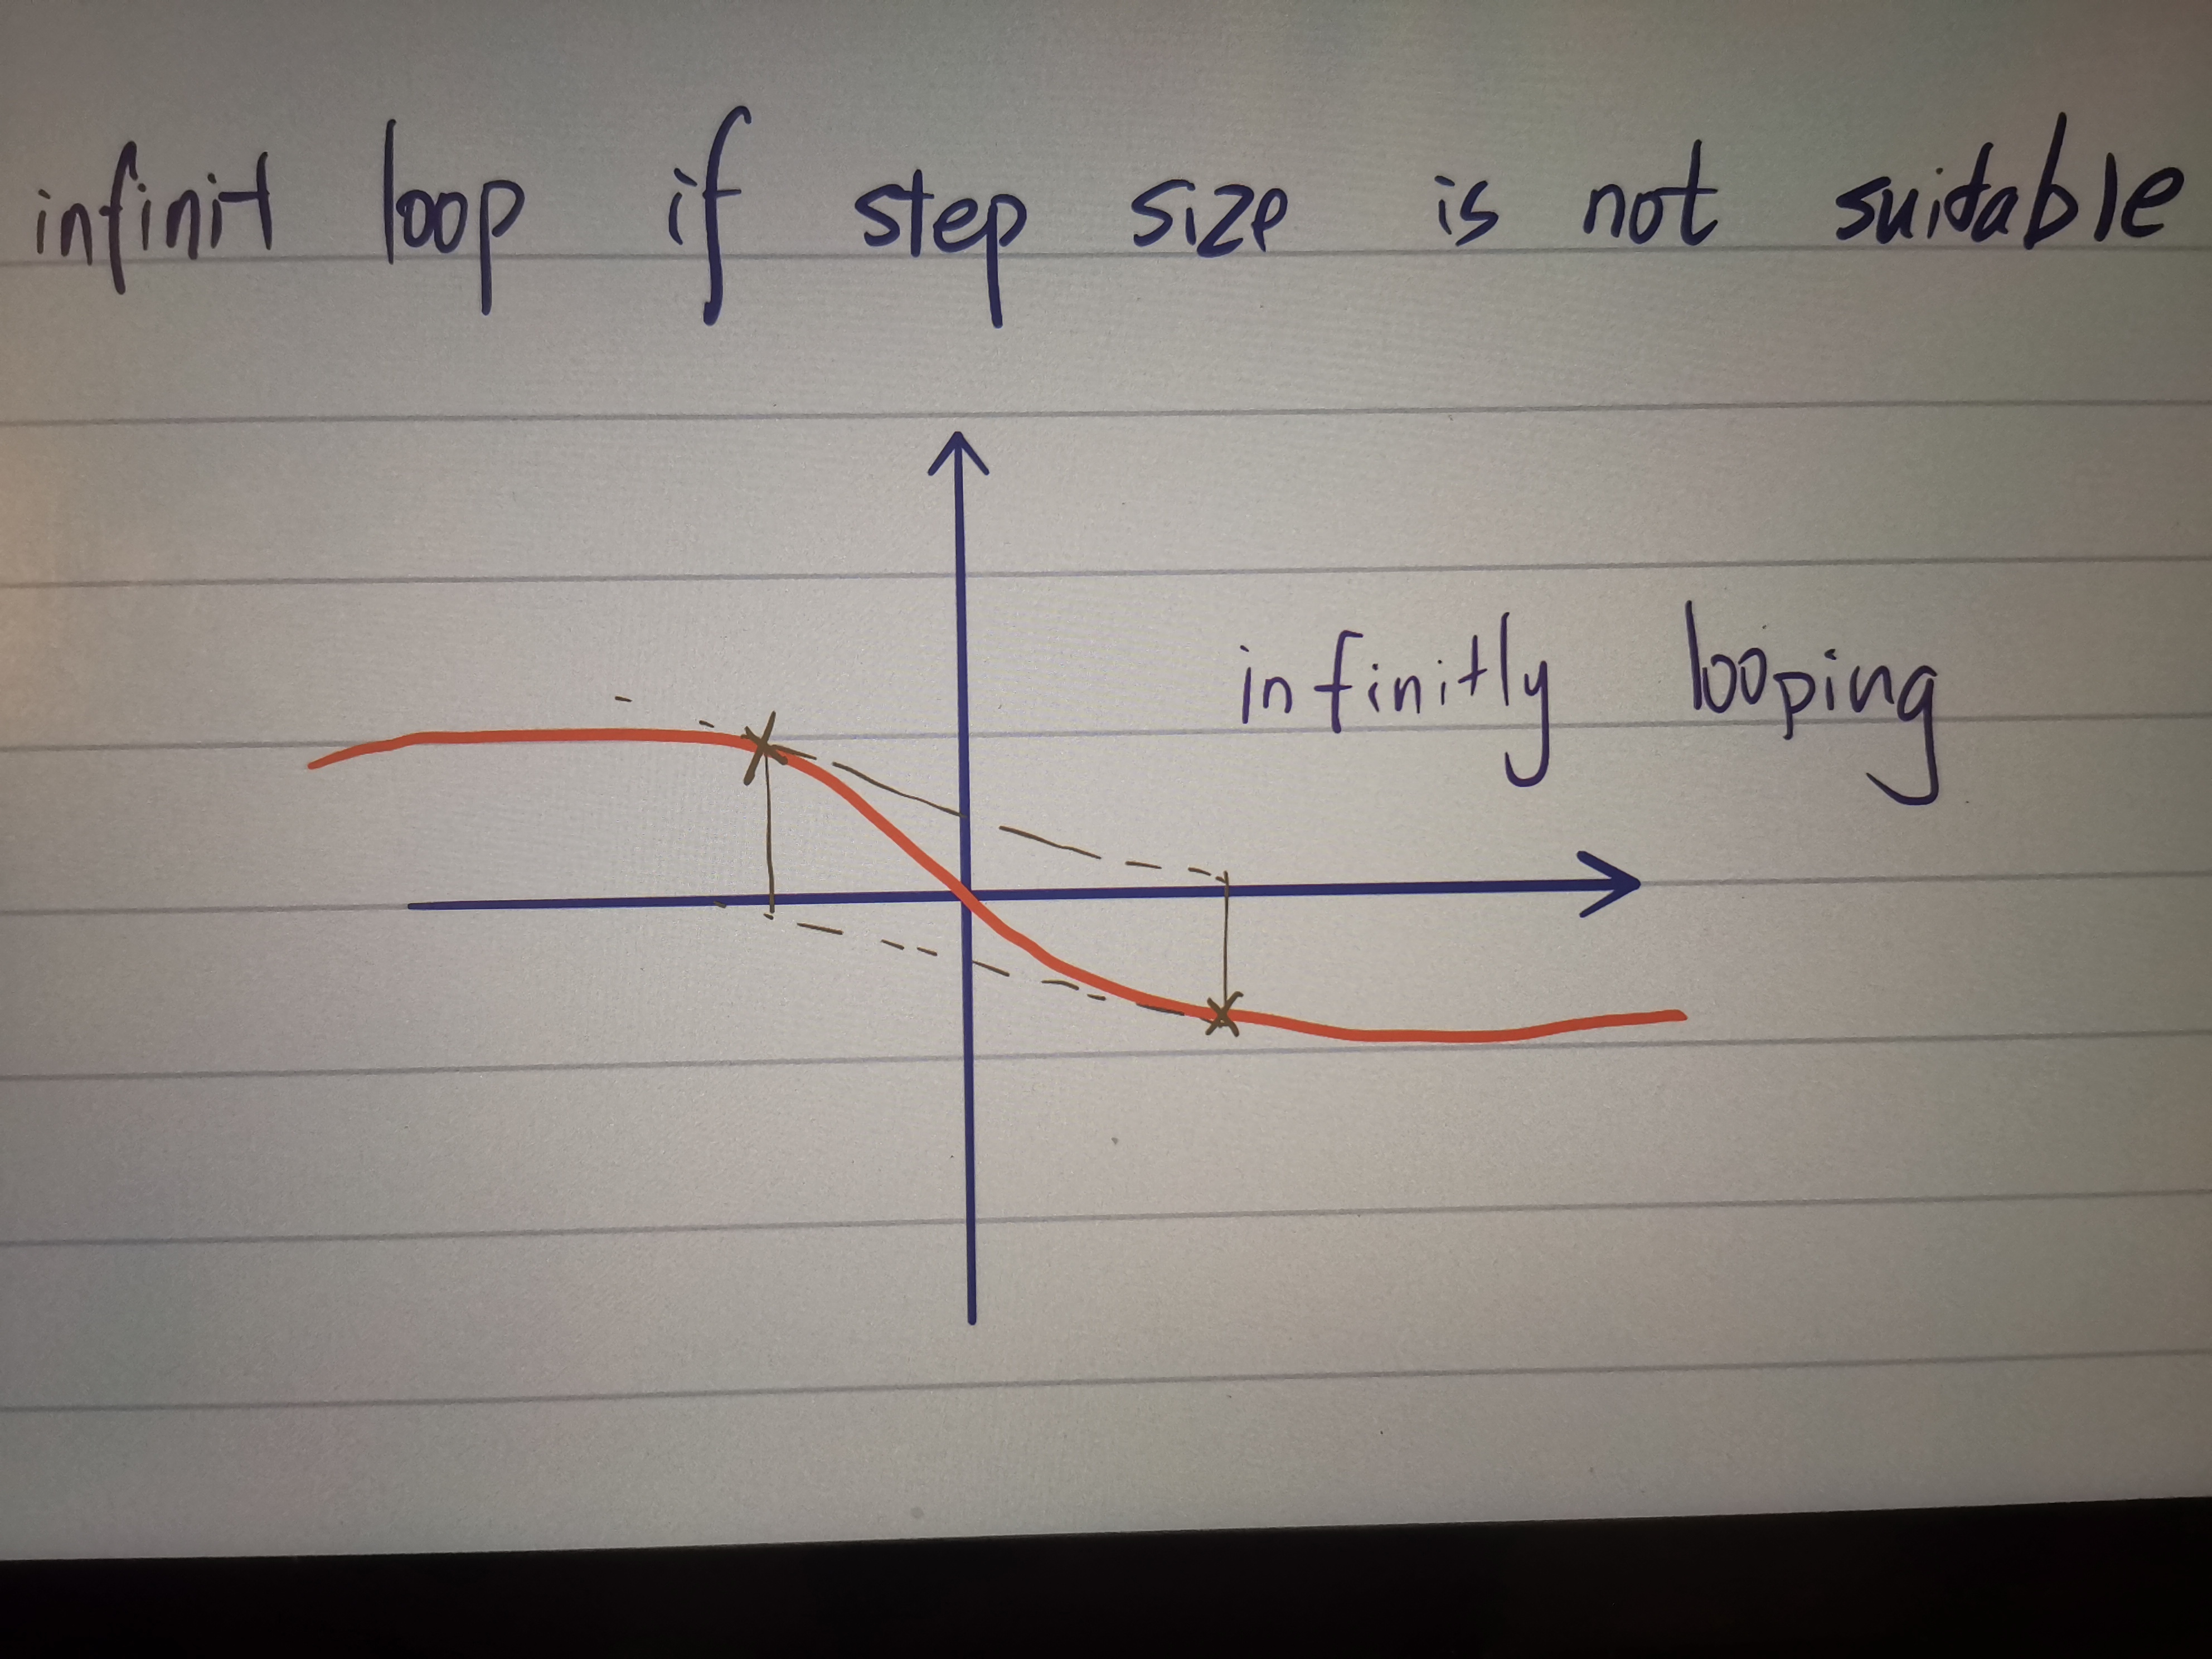
\includegraphics[width = 8cm, height = 8cm]{../code/A0_step.jpg}\\ 

\end{proof}

\begin{proof}
        (e). The expected value of the gradient of the randomly selected $m$ rows is proven to have the same expected value as the using the full gradient descent, therefore SGD is expected to work as well.\\
\end{proof}

\begin{proof}
        (f).\\
        \textbf{Upside}: SGD is much faster than calculating GD especially when the matrix of the objective function is huge.  \\
        \textbf{Downside}: if the randomly selected rows of of the weight matrix is small, it is likely that the SGD deviate from the true gradient, which will lead to reaching convergence using much more iterations.
\end{proof}
\newpage
\section*{A1}
\subsection*{Problem A1 (a)}
\begin{proof}
        To prove that $f(x) = \sum_{n=1}^{\infty} |x_i|$ is a norm, we need to prove the following: \\
        1) non-negativity: \\
        \indent i) if for all $x_i \in \mathbf{x}$, $|x_1| > 0$, then, the sum $f(\mathbf{x}) = \sum_{n=1} |x_i| > 0$. \\
        \indent ii) $\mathbf{x} = \mathbf{0} \implies $ $f(\mathbf{x})=0$\\
        \indent iii) if $\forall |x_i|\geq  0$, $f(\mathbf{x}) =  \sum_{n=1}|x_i| = 0 $ $\implies \mathbf{x} = 0$  \\
 2) absolute scalability: \\
\indent  if $\mathbf{x} = (x_1,x_2,x_3,...,x_n)$, and  $(a\mathbf{x}) = (ax_1,ax_2,ax_3,...,ax_n)$\\
\indent $f(a\mathbf{x}) = \sum_{n=1} a|x_i| = a \sum_{n=1} |x_i| = a f(\mathbf{x})$ \\ 
3) triangle inequality: \\
\indent if $\mathbf{x} = (x_1,x_2,x_3,...,x_n)$, and $\mathbf{y} = (y_1,y_2,y_3,...,y_n)$, notice that $|x_i + y_i| \leq  |x_i| + |y_i|$, then \\\
\[
\begin{aligned}
        f(\mathbf{x} + \mathbf{y}) &= f ((x_1+y_1,x_2+y_2,....,x_n+y_n)) = \sum_{i=1}^{i =n} |x_i + y_i| \\ 
                                   & \leq \sum_{i=1}^{i =n} |x_i| + |y_i|  = \sum_{i=1}^{i =n} |x_i| +\sum_{i=1}^{i =n} |y_i| = f(\mathbf{x}) + f(\mathbf{y}) 
\end{aligned}        
\]
\end{proof}
\subsection*{Problem A1 (b)}
\begin{proof}
       prove by contradiction: \\ 
       one counter example is: take $\mathbf{x} = (\frac{1}{2},0)$, $\mathbf{y} = (0,\frac{1}{2})$, therefore, $\mathbf{x+y} = (\frac{1}{2},\frac{1}{2})$
       $$g(\mathbf{x+y}) = g((\frac{1}{2},\frac{1}{2})) = (\sqrt{\frac{1}{2}} + \sqrt{\frac{1}{2}} ) ^2 = \sqrt{2}^2  = 2 $$
       $$g(\mathbf{x}) + g(\mathbf{y}) = 2* \sqrt{\frac{1}{2}}^2 = 1 $$
       because, $g(\mathbf{x+y}) \geq g(\mathbf{x}) + g(\mathbf{y})$, it vialates the traingle inequality rules in the definition. Thus,it is not a norm 


\end{proof}

\newpage
\section*{B1}
\begin{proof}
        To prove $\|x\|_{\infty} \leq \|x\|_{2} \leq \|x\|_1$
        it is essential to prove for $\mathbf{x} = (x_1,x_2,....,x_n)$:\\
        1) $\|x\|_{2} \leq \|x\|_1$\\
        2)  $\|x\|_{\infty} \leq \|x\|_{2} $\\

\noindent        prove 1) :\\
due to that $\|x\|_2 \geq 0, \|x\|_1 \geq 0$, I know that if 
$\|x\|_2^2 \leq \|x\|_1^2 \implies \|x\|_2 \leq \|x\|_1 $
\[
        \begin{aligned}
                \|x\|_1^2 & = (\sum_{i=1}^{n}|x_i|)^2 = (|x_1|+|x_2|+|x_3|+|x_4|+....+|x_n|)^2 \\
                          & \geq |x_1|^2 +|x_2|^2 + |x_3|^2+....+|x_n|^2 = \sum_{i=1}^{n} |x_i|^2 = \|x\|_2^2 \\
                          & \text{(this stands is because $|x_i|\geq 0)$          }
        \end{aligned}
        \]
therefore, $\|x\|_2^2 \leq \|x\|_1^2 \implies \|x\|_2 \leq \|x\|_1  $ \\

\noindent prove 2) \\
Suppose that every entry of $x=(x_1,x_2,...,x_n)$ is bounded, then we can write that $$\|x\|_{\infty} \leq max(x_1,x_2,....,x_n) = x_k$$ $$\|x\|_{\infty}^2 = |x_k|^2$$    
it can be seen (when proving 1) that : $$\|x\|_{2}^2 =  \sum_{i=1}^{n} |x_i|^2  = |x_k|^2 + \sum_{i \neq k} |x_i|^2 = \|x\|_{\infty} + \sum_{i \neq k} |x_i|^2 \geq \|x\|_{\infty}^2 $$
from the above, we see that $\|x\|_{\infty} \leq   \|x\|_{2}$\\

\noindent To conclude: 
$\|x\|_{\infty} \leq \|x\|_{2} \leq \|x\|_1$
\end{proof}

\newpage

\section*{A2}
\begin{proof}
        
For a set A, and $\mathbf{x} \in A$, $\mathbf{y} \in A$, if we know that $z = \lambda \mathbf{x} + (1- \lambda) \mathbf{y} \in A, \forall \lambda \in [0,1]$, then we can say that A is a convex set. That is being said if A is a convex set, any point lies on the line that connected any other two points in the set should also be in the set.\\
I: This is not a convex set.If connect point b and c, we will realize that there are points that lies out side of the set.\\

\noindent II: this is a convex set\\

\noindent III:  This is not a convex set.If connect point b and c, we will realize that there are points that lies out side of the set. \\


\end{proof}
\newpage
\section*{A3}
\begin{proof}
        conclusions are below: \\

        \noindent (a)YES.\\
         
        \noindent (b)NO\\
        if take a look at $f(x \in [a,b])$, we will realize that function value on the curve is $f(\lambda x + (1-\lambda)y) \geq (\lambda f(x) + (1-\lambda)f(y)), \forall x,y \in [a,b] $\\

        \noindent (c) NO\\
        functon value in the interval $x \in [a,c]$ violates the rule. same reasoning as (b)\\

        \noindent (d)YES \\

\end{proof}

\newpage

\section*{B2}

\begin{proof}
        (a).\\       
        to prove $f(x) = \|x\|$ is a convex function, we need to show that it obeys the rule of the definition: $$f(tx +(1-t)y) \leq tf(x) +(1-t)f(y)$$
        knowning that $f(x)$ is a norm, by definition of norm, I know: $$f(x+y) \leq  f(x) + f(y)$$
        therefore I know that: 
        \[
\begin{aligned}
        f(tx +(1-t)y) &= \|tx + (1-t)y\| \\
                      &\leq \|tx\| + \|(1-t)y\| = \leq t\|x\| + (1-t)\|y\| \\
                      &=tf(x) +(1-t)f(y)
\end{aligned}
        \]
        therefore, the function $f(x)$ is convex\\
\end{proof}


\begin{proof}
(b)\\
the goal is to show $A= \{x \in \mathbb{R}^d\}: \|x\| \leq 1\}$\\
consider two points $x,y \in A$, meaning $\|x\| \leq  1$ and 
$\|y\| \leq 1$, $\forall x,y \in A$, I am trying to prove $\|(1-t)x +ty \| \leq  1, \forall t \in [0,1]$ \\

\noindent starting off by defining point: $z =(1-t)x + ty  $:\\
\[
\begin{aligned}
        \|(1-t)x + ty \| &\leq  \|(1-t)x\| + \|ty \| \\
                         &= (1-t) \|x\| + t \|y\| \\
                         &  \leq (1-t) *max(\|x\|) + t *max(\|y\|)\\
                         &= (1-t) * 1 + t *1 = 1
\end{aligned}
\]
therefore $\|z\|=  \|(1-t)x + ty \|  \leq 1, \forall x,y \in A, t \in[0,1]$. Hence $z \in A$. A is convex
\end{proof}

\begin{proof}
        (c)\\
        No it is not. if the shaded area is the set,it can clearly been seen that, any points lies on the line between any two poins on the curve lies out-size of the set.\\

        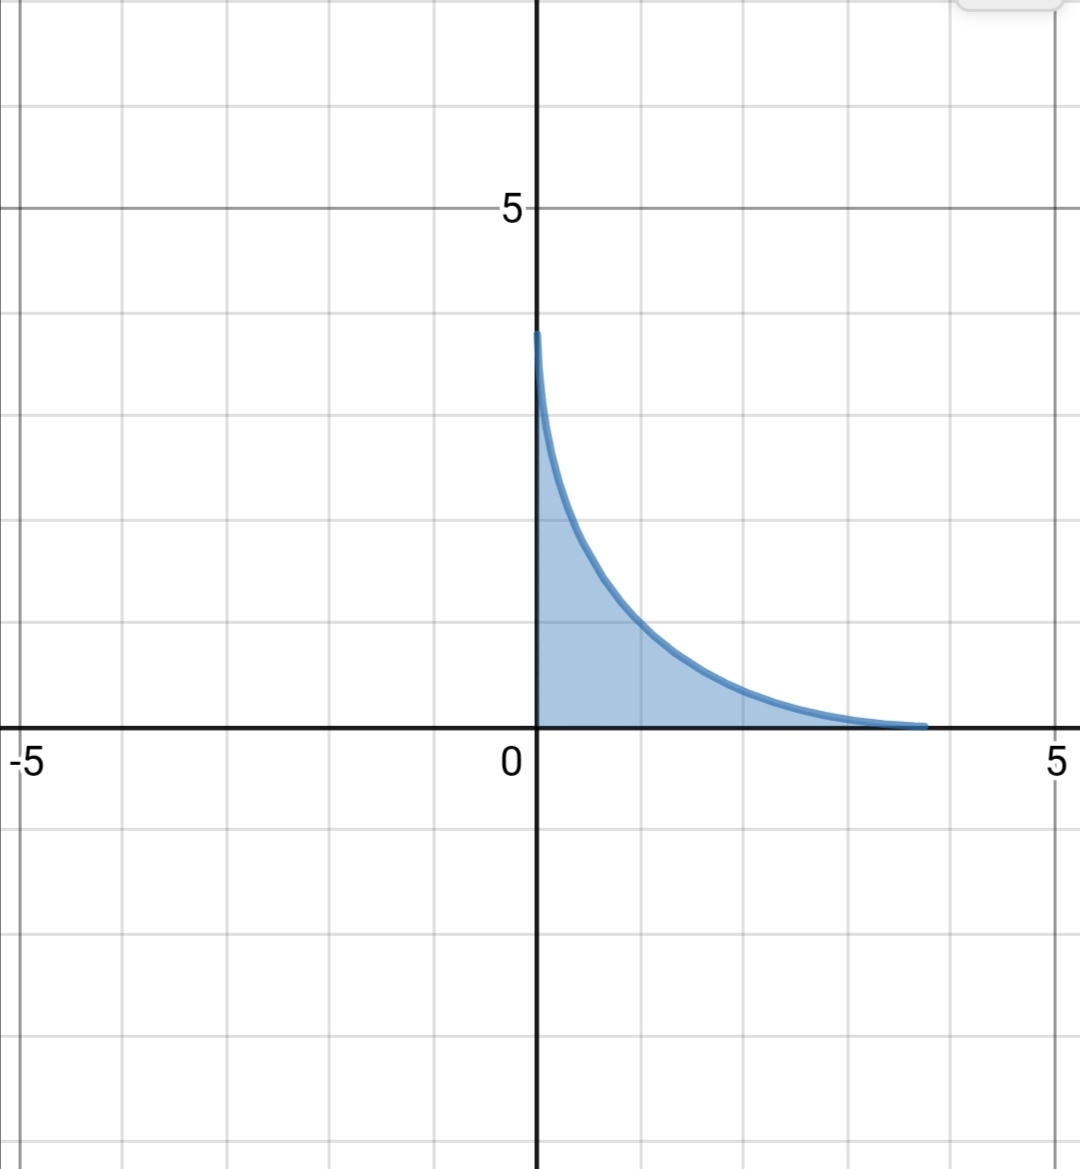
\includegraphics[width = 7cm, height = 8cm]{../code/b2_c.jpg}
\end{proof}
\newpage

\section*{B3}
\subsection*{Problem B3 (a)}
\begin{proof}
        it is known $l_i(w) for \forall i$, and $\|w\|$ are convex. Then we know that if taken $w_1, w_2 \in \mathbb{R}^d,$. Then I know that $$l_i(tw_1 + (1-t)w_2) \leq  tl_i(w_1) + (1-t)l_i(w_2)$$
        and by the definition of a norm: 
        $$\lambda \|tw_1 + (1-t) w_2\| \leq  \lambda(t\|w_1\|+ (1-t) \|w_2\|) $$
        Moreover, I know that summing up the $l_i for \forall i \leq n$ is also convex: \\
        \[
\begin{aligned}
        f(tw_2 + (1-t)w_2) &= \sum_{i=1}^n l_i(t w_1 + (1-t) w_2) + \lambda \|tw_1 + (1-t) w_2\|\\ 
                           & \leq  \sum_{i=1}^n tl_i(w_1) + (1-t)l_i(w_2) +   \lambda(t\|w_1\|+ (1-t) \|w_2\|) \\
                           & = t(\sum_{i=1}^n l_i(w_1)  + \lambda  \|w_1\|)+ (1-t) (\sum_{i =1} ^{n} l_i(w_2) + \lambda \|w_2\|)\\ 
                           & = t f(w_1) + (1-t) f(w_2)
\end{aligned}
\]

\noindent with the proof above, I can conclude that $\sum_{i=1} l_i(w) + \lambda \|w\|$ is convex
\end{proof} 
\subsection*{Problem B3 (b)}
\begin{proof}
        convex functions has nice properties like it guarantees us to find a local extrma.
\end{proof}
\newpage 

\section*{A4}
\begin{proof}
        (a).\\
        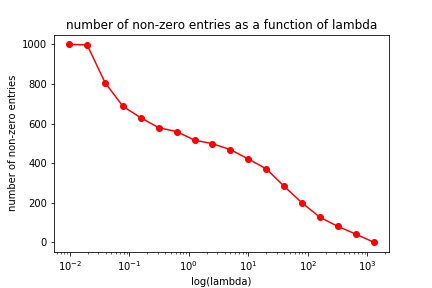
\includegraphics{../code/A4_a_linearY.png}
\end{proof}
\newpage
\begin{proof}
        (b).\\
        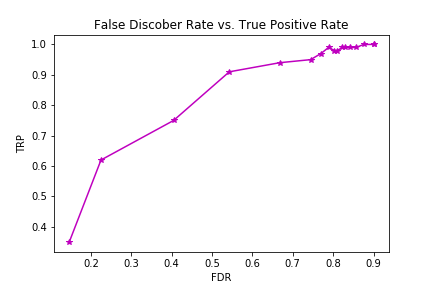
\includegraphics{../code/A4_b.png}
\end{proof}


\begin{proof}
        (c).\\

        1) from the plot in part(a), it can be seen clearly that when taking $\lambda$ to be larger than the $\lambda_{max}$, the weights are penalized to be all zeros. As $\lambda$ decreses, it starts to pick up more non-zero values. when $\lambda$ goes close to 0, meaning very little constain set on the objective function, the result is identical to the MSE solution.\\

        2) as $\lambda$ decreses, both False discover rate and True positive rate increases. This is as expected, since when $\lambda$ is large, all the weights are 0, both the $(FDA,TPA)  = (0,0)$; as $\lambda$ decreases, more entries of w start to have values that are not 0, and it can be observe that, false discover enties and true positive entries both increase, the max value for pair is $(\frac{d-k}{d}, 1) = (0.9, 1)$ 

\end{proof}

\newpage
\section*{A5}


\begin{proof}
        A5.(a)\\     
        convergence: $\|w\|_{\infty} \leq  1e-5$ \\
        stop when: $\lambda \leq  0.01$\\
        as can be seen from the plot, when $\lambda$ is large, the entries of $W$ tends to be sparse. As it decreases, $W$ started to be populated\\

        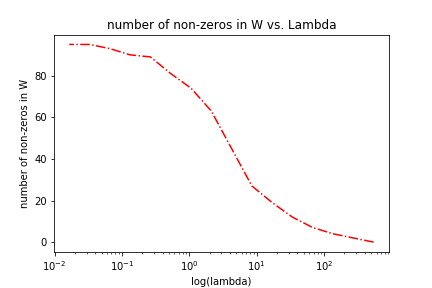
\includegraphics{../code/A5_a.png}
\end{proof}
\newpage
\begin{proof}
        A5.(b)\\     
        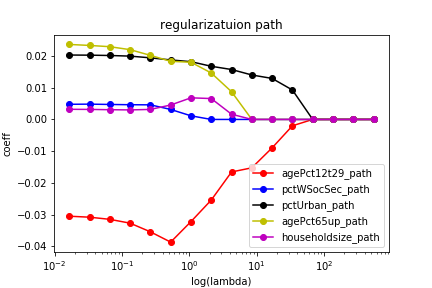
\includegraphics{../code/A5_b.png}
\end{proof}
\newpage
\begin{proof}
        A5.(c)\\     
        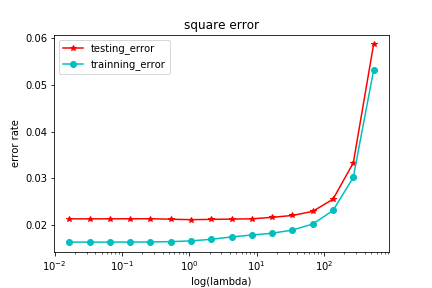
\includegraphics{../code/A5_c.png}
\end{proof}
\newpage
\begin{proof}
        A5.(d)\\     
        1)the most positive position value in w for LAMBDA=30  is0.06899592610463331, the corresponding column name is PctIlleg.\\

   \noindent     2)the most negative position value in w for LAMBDA=30  is-0.06874051933226402, the corresponding column name is PctKids2Par.\\

     \noindent    -- PctIlleg: percentage of kids born to never married (numeric - decimal)\\

\noindent -- PctKids2Par: percentage of kids in family housing with two parents (numeric - decimal)\\

\noindent -- ViolentCrimesPerPop: total number of violent crimes per 100K popuation (numeric - decimal) GOAL attribute (to be predicted)\\ 

\noindent \textbf{discussion:} as has been showned in the coefficients, percentage of kids born to be never married has a positive relation with total number of violent crimes. It is likely that, when have higher percentage of kids born to be never married, we will have a higher total number of violent crime. One thing to notice is that, there is not causul effect between the two features.       \\
For PctKids2Par, we observe that lower number of violent crimes usually associate with higher percentage of kids in family with two parents.

\end{proof}

\begin{proof}
        (e)\\     
        Although we have observed a large negative weight on 
        agePct65up, we can not say that moving people whos age are 65 up to higher crime area will \textbf{lead to} a lower crime rate, since the statistic does not tell us a causul relation. The correct way to say this is that, areas have higher percentage of people whos ages are 65 or up tends to have low crime rate. 
\end{proof}

\newpage
\section*{A6}

\subsection*{Problem A6(a)}
 \begin{proof}
         1) $\nabla_wJ(b,w) = 
\begin{bmatrix}
        \frac{d}{dw_1} J(b,w) \\
                \frac{d}{dw_1} J(b,w) \\
                \vdots \\
                        \frac{d}{dw_n} J(b,w) 
\end{bmatrix}
         $ \\
         Looking at the component inside of the sum: \\
         \[
\begin{aligned}
        (*) = & \frac{d}{dw_m} log(1 + e^{-y_i(b+x_i^Tw)}) + \lambda \|w\|_2^2 \\
              & = \frac{1}{1 + e^{-y_i(b+x_i^Tw)}} *  e^{-y_i(b+x_i^Tw)} *(-y_i x_{im})  + \frac{d}{dw_m} \lambda w^T w \\ 
        & =  \mu_i(w,b)*  e^{-y_i(b+x_i^Tw)} *(-y_i x_{im})  + 2\lambda w_m\\ 
\end{aligned}
         \]
      since we have defined $\mu_i$, we know that: \\
      $$\mu_i(w,b) =\frac{1}{1 + e^{-y_i(b+x_i^Tw)}}  \implies e^{-y_i(b+x_i^Tw)} = \frac{1}{\mu_i(w,b)}-1$$
      therefore we know that 
      $$ (*) =  \mu_i(w,b)* (\frac{1}{\mu_i(w,b)}-1) *(-y_i x_{im})  + 2\lambda w_m$$
      further more, we know\\
      $$ \frac{d}{dw_m} J(b,w) = \frac{1}{n}  \sum_{i=1}^{n} (1-\mu_i(w,b)) (-y_i x_{im}) + 2 \lambda w_m$$

\end{proof}

\begin{proof}
        2) $\nabla_bJ(w,b)$
        \[ 
\begin{aligned}
        \frac{d}{db} J(b,w) &= \frac{1}{n}      \sum_{i=1}^{n}  \frac{1}{1 + e^{-y_i(b+x_i^Tw)}} *  e^{-y_i(b+x_i^Tw)} *(-y_i )  \\ 
  &= \frac{1}{n}  \sum_{i=1}^{n} (1-\mu_i(w,b)) (-y_i) 
\end{aligned}
        \]
\end{proof}


\newpage
\subsection*{Problem A6 (b)}

$\lambda$ = .1,\\ step size=0.1,\\ tolerence=0.001
\begin{proof}
a) plotting $J(b,w)$ as a function of iteration number:

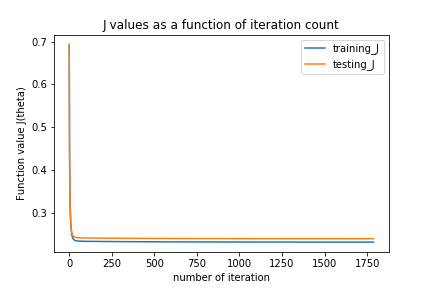
\includegraphics[width = 12cm, height = 8cm]{../code/A6_b_1.png}\\

b) error rate, with error(w\_init)=0 discarded 

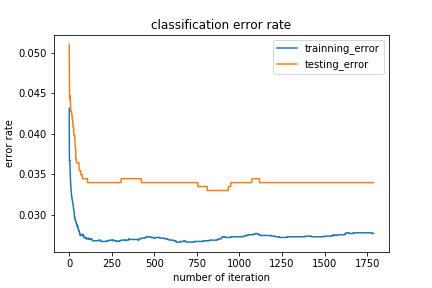
\includegraphics[width = 12cm, height = 8cm]{../code/A6_b_2.png}\\
\end{proof}

\newpage

\subsection*{Problem A6 (c)}
step size=0.01, \\tolerence=0.025
\begin{proof}
 a) plotting $J(b,w)$ as a function of iteration number:

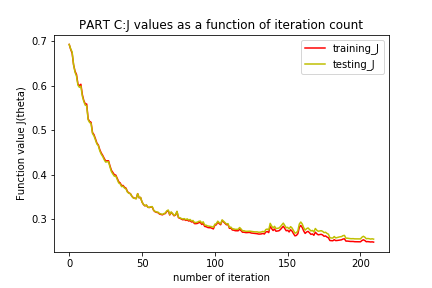
\includegraphics[width = 12cm, height = 8cm]{../code/A6_c_1.png}\\

b) error rate,with error(w\_init)=0 discarded  

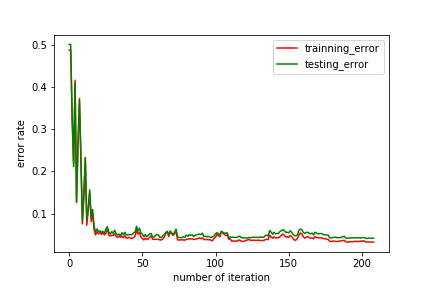
\includegraphics[width = 12cm, height = 8cm]{../code/A6_c_2.png}\\
       
               
 
\end{proof}
\newpage
\subsection*{Problem A6 (d)}
step size=0.01, \\ tolerence=0.01\\
\begin{proof}
a) plotting $J(b,w)$ as a function of iteration number:

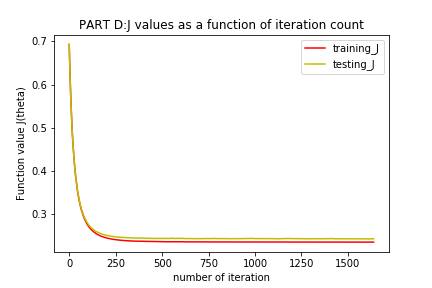
\includegraphics[width = 12cm, height = 8cm]{../code/A6_d_1.png}\\

b) error rate,with error(w\_init)=0 discarded 

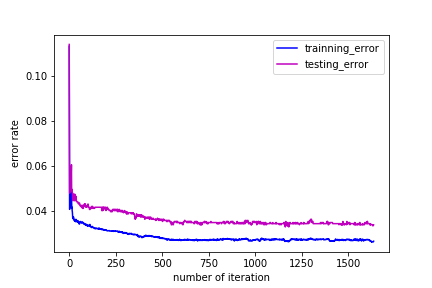
\includegraphics[width = 12cm, height = 8cm]{../code/A6_d_2.png}\\

\end{proof}

 \newpage

 \section{B4}
 \subsection*{Problem B4 (a)}
 \begin{proof}
         recall in the problem $$L(W) = - \sum_{l=1}^{k}\sum_{i=1}^{n}log(\frac{e^{w^{(l)}x_i}}{\sum_{j=1}^{k}e^{w^{(j)}x_i}}) $$
         $$\frac{d}{dw_m} L(W) = \frac{d}{dw_m}  \sum_{i=1}^{n}log(\frac{e^{w^{(l)}x_i}}{\sum_{j=1}^{k}e^{w^{(j)}x_i}}) = \sum_{i=1}^{n} \frac{d}{dw_m} log(\frac{e^{w^{(l)}x_i}}{\sum_{j=1}^{k}e^{w^{(j)}x_i}}) $$
         First, I would want to take a look at the component inside of the sum. There are 2 situations, 1) $m \neq l$,  2) $ m = l$\\

\noindent 1) when $m\neq l$\\
\[
\begin{aligned}
        (*_1)  =&  \frac{d}{dw_m} log(\frac{e^{w^{(l)}x_i}}{\sum_{j=1}^{k}e^{w^{(j)}x_i}})\\
        =& \frac{\sum_{j=1}^{k}e^{w^{(j)}x_i}}{e^{w^{(l)}x_i}}* (-1)* \frac{e^{w^{(l)}x_i}}{(\sum_{j=1}^{k}e^{w^{(j)}x_i})^2}*e^{w^{(m)} x_i}*x_i \\
         & \text{(after cancelling terms)}\\
         & = (-1) \frac{e^{w^{(m)}x_i}}{\sum_{j=1}^{k}e^{w^{(j)}x_i}} * x_i = 0 - x_i \widehat{y_i}^{(W)}\\
\end{aligned}
\]

2) when $m = l$
\[
\begin{aligned}
        (*_2)  =&  \frac{d}{dw_m} log(\frac{e^{w^{(l)}x_i}}{\sum_{j=1}^{k}e^{w^{(j)}x_i}})\\
=& \frac{\sum_{j=1}^{k}e^{w^{(j)}x_i}}{e^{w^{(l)}x_i}}*  \frac{x_ie^{w^{(m)}x_i} *\sum_{j=1}^{k} e^{x_iw^{(j)}} - x_ie^{w^{(m)}x_i} *e^{w^{(m)}x_i} }{(\sum_{j=1}^{k}e^{w^{(j)}x_i})^2}\\
         & \text{(after cancelling terms)}\\
         & = x_i - \frac{e^{w^{(m)}x_i}}{\sum_{j=1}^{k}e^{w^{(j)}x_i}} * x_i \\
         & = x_i - x_i \widehat{y_i}^{(W)}
\end{aligned}
\]

\newpage
Combine 1) and 2): \\ 
$$(*) = \frac{d}{dw_m} log(\frac{e^{w^{(l)}x_i}}{\sum_{j=1}^{k}e^{w^{(j)}x_i}})= x_i (1\{l=m\}\} - \widehat{y_i}^{W})$$
Therefore the final result is 
$$ \sum_{i=1}^{n}(*) = -\sum_{i=1}^{n} x_i (1\{l=m\}\} - \widehat{y_i}^{W})$$
$$and$$
$$\nabla_w L(W) = \sum_{i=1}^{n} -x_i (y_i- \widehat{y_i}^{W})^T$$
 \end{proof}

 \newpage
 \subsection*{Problem B4 (b)}
 \begin{proof}
         recall $J(W) - \frac{1}{2} \sum_{i=1}^{n} \|y_i - W^Tx_i\|^2$, where $\widehat{y}^{W} = W^Tx_i $ \\ 
         \[
\begin{aligned}
        \frac{d}{dw_m} J(W) &= \frac{d}{d{w_m}} \frac{1}{2} \sum_{i=1}^{n} (y_i - W^Tx_i)^T  (y_i - W^Tx_i)\\
                            &\text{by chain rule}\\
                            & = \frac{1}{2} \sum_{i=1}^{n} (\frac{d}{dw_m}(y_i - W^Tx_i))^T  (y_i - W^Tx_i) + (\frac{d}{dw_m}(y_i - W^Tx_i))  (y_i - W^Tx_i)^T)\\
                            & = -\frac{1}{2} \sum_{i=1}^{n} 2 * x_{im} (y_i - W^Tx_i)
\end{aligned}
                 \]
                therefore the full gradient is : \\ 
$$\nabla_w J(w) = -\sum_{i=1}^{n} x_i(y_i - \widehat{y}^{(W)}) $$
 \end{proof}
\newpage
 \subsection*{Problem B4 (c)}
\begin{proof}
        the parameters used: \\

    \noindent    Multinomial reg :\\ step size: 0.1\\ stopping criteria: $\|W\|_{\infty} \leq 1e-3$\\

        \noindent         MSE  :\\ step size: 0.1\\ stopping criteria: $\|W\|_{\infty} \leq 1e-3$\\


       \noindent  Final result: \\
        1) Multinomial Logistic Regression: \\

        Final \textbf{train} set  Accuracy for Multinomial Regression is : 0.9151833333333333 \\

Final \textbf{test} set Accuracy for Multinomial Regression is : 0.918\\


\noindent 2) MSE: \\

Final \textbf{trainning} set Accuracy for MSE is : 0.8448666666666667\\

Final \textbf{test} set Accuracy for Least square is : 0.8519
\end{proof} 

 
 


\end{document}
\section{Chapter 1}
\subsection*{Problem 1}

\begin{enumerate}[label=\roman*)]
  \item $a \in \Z$
  \item $A^\Trans = A$
  \ item $A\vec{v} = \lambda \vec{v}$
  \item $\One$
\end{enumerate}
pupupu $|a|=15$, pupupupu.
